\section{Introduction}
\label{sec:intro}

\begin{figure}[t]
\centering
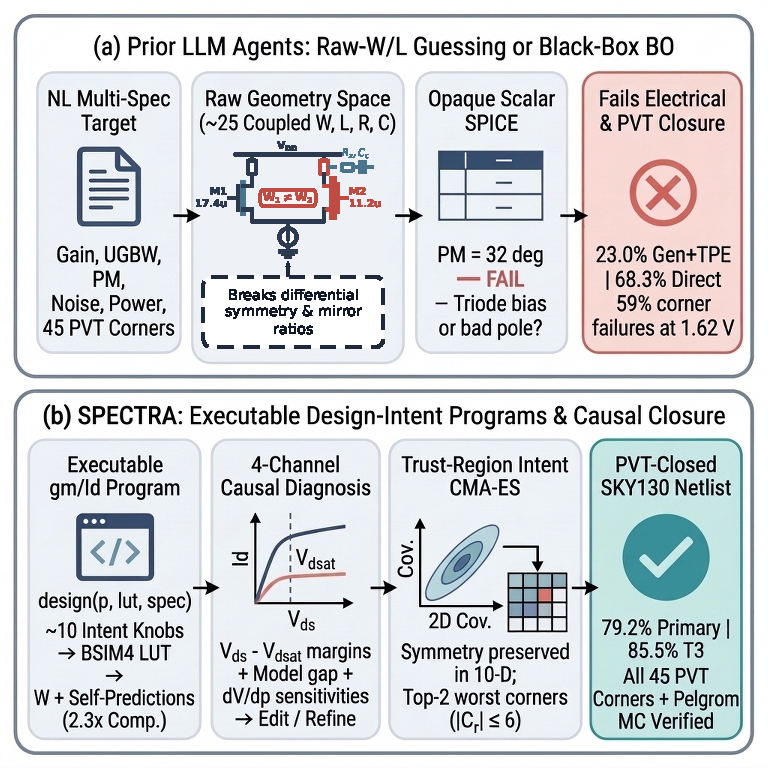
\includegraphics[width=0.99\columnwidth]{figs/spectra_teaser.pdf}
\vspace{-2.5mm}
\caption{Paradigm comparison. \textbf{(a)} Direct width generation and black-box $W/L$ optimization search a coupled ${\sim}\RawVars{}$-variable geometry space with scalar SPICE feedback, frequently failing electrical and low-$V_{DD}$ corner closure. \textbf{(b)} \textsc{SPECTRA} compiles specifications into executable $g_m/I_D$ intent programs (${\sim}\IntentVars{}$ variables, $\RawOverIntent{}\times$ compression), pairing four-channel device diagnosis with invariant-preserving trust-region CMA-ES and adaptive 45-corner PVT closure.}
\Description{Comparison of prior direct-width and black-box optimization agents against SPECTRA's executable gm/Id design-intent program and causal diagnosis loop.}
\label{fig:teaser}
\end{figure}

Analog and mixed-signal (AMS) blocks---operational amplifiers, low-dropout regulators (LDOs), bandgap voltage references, continuous-time and clocked comparators, oscillators, and active filters---form the physical interface of modern system-on-chips, yet remain resilient to full design automation~\cite{razavi2017design,allen2012cmos}. Bridging a natural-language specification to silicon-ready schematics demands tightly coupled decisions: choosing a viable circuit topology, budgeting branch currents and overdrive headroom, sizing dozens of interdependent transistors, and iterating with SPICE until all AC, DC, transient, and noise targets hold simultaneously across process, voltage, and temperature (PVT) variations and local device mismatch~\cite{pelgrom1989matching,jespers2017gmid}.

Large language models (LLMs) have recently been introduced into this design loop along two lines. Training-free code-generation agents synthesize circuit topologies as executable scripts with simulator error feedback~\cite{lai2025analogcoder,bao2026analogagent,chen2025menter} or combine topology drafting with Bayesian optimization (BO) and multi-agent role specialization~\cite{lai2026analogcoderpro,wang2025analogsage,habib2026aallm,huang2026saftac}. In parallel, fixed-topology sizing frameworks leverage LLMs to guide sample selection or subspace pruning on human-supplied schematics~\cite{yin2024adollm,kochar2025ledro,ahmadzadeh2025anaflow,yu2026autosizer,hao2026agenticsizing,long2026analogscout,saxena2026opera,park2026craft}.

Despite encouraging progress on functional netlist generation, three fundamental bottlenecks prevent existing LLM agents from achieving end-to-end electrical and multi-corner closure. \textbf{(1) Representation mismatch:} LLMs reason effectively about qualitative circuit principles---such as cascoding for output resistance, Miller nulling for phase margin, or weak-to-moderate inversion trade-offs---but perform poorly when asked to emit raw transistor widths in micrometres across ${\sim}\RawVars{}$ coupled $W/L/R/C$ parameters; conversely, handing raw geometries to unconstrained black-box BO~\cite{lai2026analogcoderpro} breaks differential symmetry, mirror ratios, and bias invariants. \textbf{(2) Diagnostic opacity:} scalar simulator pass/fail tables (e.g., reporting $\text{PM}=32^\circ$) conceal whether failure stems from a tail current source crushed into triode or an invalid analytical pole assumption, leaving the model to guess blind edits. \textbf{(3) Multi-corner closure vs.\ budget starvation:} evaluations restricted to Level-1 square-law models or nominal TT corners~\cite{lai2025analogcoder,wang2025analogsage,habib2026aallm} mask corner fragility---in our pilot on relaxed specifications, every agent saturated near $100\%$ nominal pass rate, whereas near the Pareto frontier $92\%$ of TT-passing corner failures break at low supply ($1.62\,\text{V}$), and naive full-grid SPICE evaluation inside an inner search loop rapidly exhausts simulation budgets~\cite{adbench2026longhorizon}.

To address these challenges, we propose \textbf{\textsc{SPECTRA}}---\emph{\textbf{SPEC}i\-fi\-ca\-tion-to-PV\textbf{T}-Closed \textbf{TR}an\-sis\-tor-Level \textbf{A}na\-log Syn\-the\-sis}---an end-to-end synthesis framework built around executable $g_m/I_D$ design-intent programs (Figure~\ref{fig:teaser}). Rather than generating static SPICE widths, \textsc{SPECTRA} tasks the LLM with authoring a self-predicting Python sizing procedure over low-dimensional physical intent variables---transconductance efficiencies $g_m/I_D$, channel lengths $L$, branch currents $I_D$, and compensation ratios---mapped deterministically to device geometries through pre-characterized BSIM4 lookup tables. A four-channel causal diagnosis engine inspects device operating-point margins ($V_{DS}-V_{dsat}$), discrepancies between the program's own analytical predictions and SPICE measurements, and finite-difference intent sensitivities to route a hierarchical repair policy between structural program edits and invariant-preserving trust-region CMA-ES, coupled with adaptive worst-corner active-set expansion across 45 PVT conditions.

Our main contributions are summarized as follows:
\begin{itemize}[leftmargin=*, topsep=2pt, itemsep=1.5pt]
\item \textbf{Executable Intent Synthesis and Invariant Search.} We formulate transistor-level synthesis as generating self-predicting $g_m/I_D$ sizing programs backed by multi-corner BSIM4 lookup tables, compressing the optimization space by $\RawOverIntent{}\times$ (median \IntentVars{} intent variables vs.\ \RawVars{} raw device dimensions) while preserving matching and biasing constraints throughout trust-region CMA-ES refinement.
\item \textbf{Device-Level Causal Diagnosis and Adaptive PVT Closure.} We design a deterministic four-channel analyzer that couples operating-region margins, model-to-SPICE prediction gaps, and intent sensitivities with a hierarchical \textsc{Edit}/\textsc{Refine}/\textsc{Declare} policy and worst-corner active-set promotion, cutting simulation work by $24.6\%$ while closing 45-corner PVT targets.
\item \textbf{\textsc{SPECTRA-Bench} and Comprehensive Multi-Track Evaluation.} We release \textsc{SPECTRA-Bench} (\NTasksTotal{} tasks across \NPrimaryFamilies{} SKY130 circuit families with Pareto-refined feasibility certificates, 25 independent practitioner tasks, 45-corner PVT, and Pelgrom mismatch verification). Across end-to-end synthesis, a 166-case fault-injection suite, an eight-framework external sizing benchmark (36- and 92-task matrices), and cross-simulator (\texttt{ngspice}/\texttt{Xyce}) and cross-PDK (\texttt{GF180MCU}/\texttt{ASAP7}) tracks, \textsc{SPECTRA} reaches \SpectraPrim{} end-to-end primary success (\SpectraTThree{} on near-frontier T3) and reveals sharp physical boundaries of analytical self-prediction and standalone LLM fault localization.
\end{itemize}
